\chapter{Recolección de datos de tráfico}
\label{cap:3}

Actualmente existen una variedad de tecnologías para la recolección automática de datos del tráfico. Según Mimbela \cite{mimbela2003summary} podemos dividir estas tecnologías en dos. La primera es la \emph{tecnología in-situ}, que toma los datos del tráfico a través de detectores ubicados a lo largo del camino y que vuelve a dividirse en dos categorías: la intrusiva y la no intrusiva. La segunda, denominada \emph{Floating Car Data} (FCD), es una alternativa para obtener datos del tráfico de gran calidad mediante el uso de vehículos sonda equipados con dispositivos de medición que pueden ser dedicados o no.

\section{Tecnologías in-situ}

Las \emph{tecnologías de detección in-situ} se basan en la recolección de datos mediante dispositivos específicos para este fin que son dispuestos físicamente en los lugares sujetos de medición. Se dividen en dos categorías: \begin{enumerate*}[a)] \item las tecnologías \emph{intrusivas}, que están montadas en o por debajo de la superficie de las rutas y cuya instalación ocasiona la interrupción potencial del tráfico y \item las tecnologías \emph{no intrusivas}, que son montadas encima o sobre la superficie de las rutas y su instalación no genera interrupción del tráfico o lo hace en pequeña medida.\end{enumerate*}

\subsection{Sensores de tecnología intrusiva}

Los tipos de sensores y la ubicación de los mismos se pueden observar en la \Cref{fig:intrusiva}. El primer tipo de unidades son los \emph{sensores magnéticos pasivos} o  \emph{magnetómetros} que pueden ser montados de forma permanente en hoyos a lo largo del camino, o pegados a la superficie de la ruta. Estas unidades se comunican a una estación de procesamiento cercana utilizando cables debajo del camino o a través de comunicación inalámbrica. El sensor tiene una zona circular o elíptica de alcance de detección. Los magnetómetros monitorean la fluctuación en la fuerza dentro de un campo magnético generado, el cual cambia en presencia de objetos de metal moviéndose a través del mismo.

\begin{figure}[h]
	\centering
	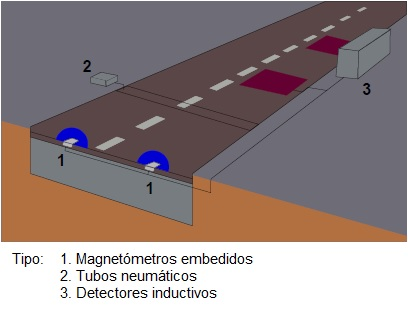
\includegraphics[width=0.7\textwidth]{capitulos/3/figuras/figura1.jpg}
	\caption{\label{fig:intrusiva} Típicas configuraciones de detección intrusiva}	
	%TODO cambiar el texto 3 del gráfico por Detectortes de inducción %
\end{figure}

Un segundo tipo de unidades utiliza \emph{tubos neumáticos} que son extendidos a través de la calzada y que se fijan en la acera en ambos extremos. Una ráfaga de presión de aire se produce en el tubo de goma cuando un vehículo pasa por encima. El pulso de presión de aire cierra un interruptor produciendo una señal eléctrica que es transmitida.

El tercer tipo son los \emph{detectores de bucle de inducción}, que consisten en rollos de alambre recubierto, enterrados en ranuras cortadas en la superficie de la carretera y sellados con masilla. Los datos son enviados a través de un cable enterrado con los bucles hasta una unidad de procesamiento. Una señal eléctrica es aplicada al bucle, la cual oscila en presencia de un vehículo en movimiento. Estos cambios son detectados por la unidad de procesamiento que genera un evento que es transmitido.

Otro tipo de detector intrusivo, denominado \emph{weigh-in-motion} mostrado en la \Cref{fig:Weight-In-Motion}, consisten en un sensor piezoeléctrico ubicado en un canal a través del camino. El sistema registra la variación de tensión medida en los piezoeléctricos, lo cual genera un evento que es transmitido para su procesamiento. Estos sistemas  se utilizan en ubicaciones específicas mayormente para el control de acceso.

\begin{figure}[h]
	\centering
	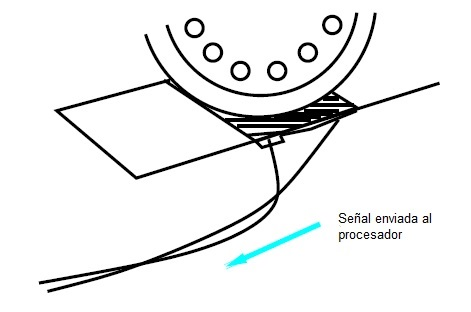
\includegraphics[width=0.7\textwidth]{capitulos/3/figuras/figura2.jpg}
	\caption{\label{fig:Weight-In-Motion}  Sistema de detección weight-in-motion}	
\end{figure}

\subsection{Sensores de tecnología no intrusiva}

Los sensores de tecnología no intrusiva incluyen:  recolección de datos por video, detectores infrarrojos pasivos o activos, radares de microondas, detectores ultrasónicos, detectores acústicos, detectores láser y fotografía aérea. La mayoría de los sistemas no intrusivos son operacional y visualmente similares, consistiendo en pequeñas unidades electrónicas montadas en contenedores a prueba de agua.

\begin{figure}[h]
	\centering
	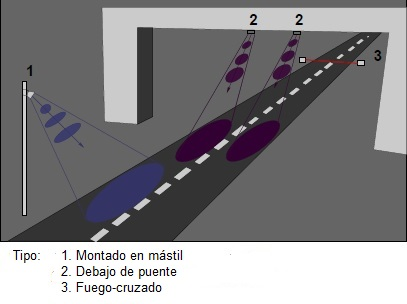
\includegraphics[width=0.7\textwidth]{capitulos/3/figuras/figura3.jpg}
	\caption{\label{fig:noIntrusica}  Configuraciones típicas de tecnologías no intrusivas}	
\end{figure}

En la \Cref{fig:noIntrusica} pueden notarse una disposición de 3 tipos de deterctores no intrusivos. El primer tipo corresponde a los \emph{montados en mástil} al costado de la carretera, tales como cámaras fotográficas o de video, capaces de procesar un campo de visión que cubre un área oblicua.  Problemas de oscurecimiento pueden ocurrir cuando vehículos grandes cubren a vehículos pequeños o cuando el campo de visión es muy grande, causando la detección de vehículos fuera del carril deseado.

El segundo tipo de detectores no intrusivos son los \emph{montados debajo de puentes o portales}, con un campo de visión justo por debajo de los mismos, o ligeramente oblicuo a la unidad. Este tipo de detectores también está sujeto a los problemas mencionados anteriormente.

Finalmente, el tercer tipo, conocidos como de \emph{fuego cruzado}, consiste en unidades, tales como monitores de polución, que son montados a nivel del piso a ambos lados del camino, disparando un haz a través de la carretera. Estas unidades están sujetas al enmascaramiento de lado a lado, por lo tanto, son más adecuadas para un solo carril.

\section{Tecnologías de Floating Car Data}

Además de la utilización de tecnologías in-situ, muchas aplicaciones de gestión de tráfico utilizan dispositivos montados en vehículos en circulación, conocidos como sistemas de ubicación automática de vehículo (\emph{Automatic Vehicle Location} - AVL). Los dispositivos AVL pueden proveer dos tipos de información: \begin{enumerate*}[a)]
\item información de posición, cuando un vehículo equipado con ellos pasa cierto punto de la red donde existe un sensor, o \item información continua, a medida que el vehículo transita a través de la red, en este caso el dispositivo AVL cuenta con una conexión dedicada para transmitir activamente los eventos.
\end{enumerate*}

Los primeros sistemas AVL se basaron en vehículos equipados con transpondedores que transmitían y recibían información de los dispositivos de control ubicados en la carretera. Los dispositivos AVL actuales se basan principalmente en la tecnología del Sistema de Posicionamiento Global (\emph{Global Positioning Systen} - GPS). Los vehículos sonda pueden ser equipados con dispositivos AVL dedicados o incluso se pueden utilizar dispositivos móviles, tales como teléfonos celulares, para que momentáneamente actúen como dispositivos AVL cuando su usuario viaja en vehículo.  

Un sistema basado en FCD consiste en recolectar y procesar datos de tráfico obtenidos en tiempo real a través de dispositivos AVL montados en vehícuos que circulan en una red de caminos sujeta a observación, como se muestra en la \Cref{fig:ComunicacionGPS}. Todos los vehículos equipados con estos dispositivos actúan como sensores dentro de la red de caminos. Datos como la ubicación del vehículo, la velocidad y dirección del viaje son enviados a un centro de procesamiento de información. Luego de la recolección y extracción de los datos, información útil como el estado del tráfico y rutas alternativas pueden ser derivadas y posteriormente distribuidas.

\begin{figure}[h]
    %TODO crear nueva figura
	\centering
	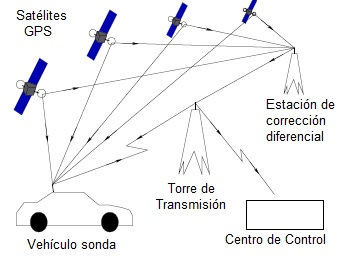
\includegraphics[width=0.7\textwidth]{capitulos/3/figuras/figura4.jpg}
	\caption{\label{fig:ComunicacionGPS} Esquema típico de recolección de datos mediante FCD}	
\end{figure}

\subsection{FCD basado en GPS}

Hoy en día la tecnología GPS se encuentra altamente disponible, lo que se refleja en el aumento del número de vehículos y dispositivos móviles equipados con este sistema de ubicación. Esto lleva al desarrollo de trabajos que aprovechan esta tecnología para la implementación de sistemas basados en FCD tales como  \cite{giovannini2011novel,li2007practical,sevlian2010travel,yin2004weight}

En \cite{giovannini2011novel} se utilizan vehículos sonda particulares con GPS integrado, la toma de posiciones puede funcionar en dos modos: \begin{enumerate*}[1)] \item el modo standard donde el dispositivo toma y almacena posiciones cada 2 km, luego de almacenar 50 posiciones, las envía a un servidor. \item El modo información de tráfico donde se toman posiciones cada 30 segundos y se envían al servidor una vez que se tengan 24 posiciones almacenadas.\end{enumerate*}

En \cite{sevlian2010travel} se utilizan taxis equipados con GPS que toman localizaciones cada 2 minutos junto con información histórica de las rutas y un algoritmo de aprendizaje de máquinas para predecir tiempos de viaje.


%TODO describir algunos trabajos citados.

\subsection{FCD basado en dispositivos móviles}

La rápida expansión de los teléfonos y dispositivos inteligentes, y los múltiples sensores que actualmente poseen los mismos, los convierte en potenciales dispositivos AVL utilizables para la implementación de sistemas basados en FCD. Muchos trabajos se centran en la utilización de dispositivos móviles para la detección del tráfico, la mayoría aprovechando los sensores A-GPS\footnote{http://es.wikipedia.org/wiki/GPS\_Asistido} disponibles en los mismos, como también existen otros que utilizan las redes GSM\footnote{http://en.wikipedia.org/wiki/GSM}, WiFi\footnote{http://en.wikipedia.org/wiki/Wi-Fi} e incluso con tecnología Bluetooth\footnote{http://en.wikipedia.org/wiki/Bluetooth} \cite{thiagarajan2010cooperative,thiagarajan2009vtrack,fraser2007use,fang2011enacq,ruppe2012augmenting}.

En 2007, Fraser \cite{fraser2007use} habla de la viabilidad de utilización de dispositivos móviles como alternativa a los métodos típicos de detección de tráfico, utilizando ubicación de objetos mediante triangulación con antenas de telefonía, tal como se muestra en la \Cref{fig:triangulacionAntenas}. En el mismo trabajo se mencionan las dificultades que tienen tales sistemas en cuanto a la precisión de ubicación, quedando este punto como una problemática a ser resuelta.

\begin{figure}[h]
%TODO cambiar al español
	\centering
	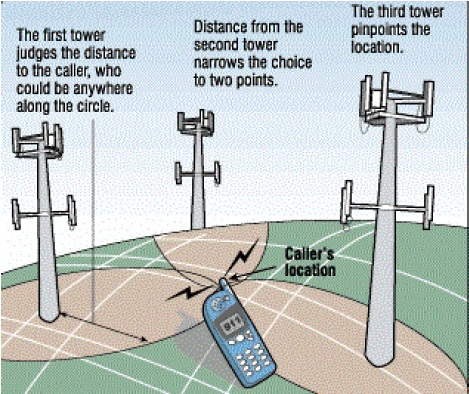
\includegraphics[width=0.7\textwidth]{capitulos/3/figuras/figura5.jpg}
	\caption{\label{fig:triangulacionAntenas} Triangulación de Antenas}	
\end{figure}

A pesar de la baja precisión de los sistemas GSM para la ubicación de dispositivos móviles, se ha propuesto un trabajo denominado CTrack \cite{thiagarajan2011accurate}, que utiliza la red GSM y otros sensores disponibles en el teléfono para la ubicación y obtención de información de FCD. El sistema consiste en dos componentes de software, una librería para el teléfono y un servicio en la web. La librería recolecta, filtra y escanea los datos obtenidos con el teléfono y los transmite a través de la red inalámbrica al servicio web, el cual corre un algoritmo de \emph{Map Matching} con los datos recibidos para identificar las vías en utilización. El trabajo comentado tiene como premisa hacer un uso eficiente del consumo de la batería del dispositivo, evitando usar sensores de alto consumo tales como el sensor GPS o la antena WiFi.

Otro trabajo sobre FCD y que también busca un uso eficiente de energía se denomina EnAcq \cite{fang2011enacq}. El mismo propone un método de adquisición de ubicaciones por medio de GPS y luego realiza un proceso de \emph{Map Matching} mejorado para procesar datos de poca precisión. Para evitar el consumo innecesario de energía, utiliza una estrategia adaptativa de toma de ubicaciones que se basa en detectar el estado de movimiento del dispositivo.

Ruppe\cite{ruppe2012augmenting} presenta una propuesta que utiliza las tecnologías Bluetooth y WiFi para detectar la ubicación de los vehículos u otros objetos sensibles de tráfico. Su enfoque se basa en la ubicación indirecta de los objetos sensibles de tráfico (autos, ciclistas y transeúntes) mediante el uso de sensores fijos y móviles que detectan los dispositivos con WiFi o Bluetooth activados que poseen estos objetos. Por ejemplo, un vehiculo que actúa como sensor móvil está equipado con receptores específicos que detectan todos los objetos de tráfico que están dentro de su área de alcance, recolentando la identificación de WiFi o Bluetooth de los mismos. Los datos medidos son procesados y permiten obtener trayectorias, tiempos de viaje, estado del tráfico y matrices de origen-destino así como otros datos acerca del tráfico.
